%=========================================================
% Step-by-Step Handout : Git and GitHub with VS Code
% Modern Computing and Python Programming (26ESCC106)
% Compile using XeLaTeX:
%   latexmk -xelatex -interaction=nonstopmode -halt-on-error git-github-handout.tex
%=========================================================

\documentclass[11pt,a4paper]{article}

%---------------------------------------------------------
% Packages
%---------------------------------------------------------
\usepackage[margin=2cm,headheight=28pt,headsep=12pt]{geometry}
\usepackage{fontspec}
\setmainfont{Times New Roman}
\usepackage{amsmath,amssymb}
\usepackage{graphicx}
\usepackage{booktabs}
\usepackage{array}
\usepackage{tabularx}
\usepackage{enumitem}
\usepackage{fancyhdr}
\usepackage{xcolor}
\usepackage{listings}
\usepackage[most]{tcolorbox}
\usepackage{tikz}
\usetikzlibrary{arrows.meta,positioning,shapes.geometric,shapes.misc,fit,calc,decorations.pathreplacing}
\usepackage[hidelinks]{hyperref}
\usepackage{titlesec}

\setlist{itemsep=2pt,topsep=3pt,leftmargin=*}
\setlength{\parindent}{0pt}
\setlength{\parskip}{5pt}
\setlength{\emergencystretch}{1.5em}

%---------------------------------------------------------
% Header / Footer
%---------------------------------------------------------
\pagestyle{fancy}
\fancyhf{}
\fancyhead[L]{
\includegraphics[height=22pt]{images/MITE_logo.png}}
\fancyhead[C]{\small\textbf{Modern Computing and Python Programming (26ESCC106)}\\ \footnotesize Handout: Git and GitHub with VS Code}
\fancyhead[R]{\small Manjunath Prasad H. R.}
\fancyfoot[C]{\small Page \thepage}
\renewcommand{\headrulewidth}{0.6pt}

%---------------------------------------------------------
% Headings
%---------------------------------------------------------
\titleformat{\section}{\Large\bfseries}{\thesection.}{0.5em}{}
\titleformat{\subsection}{\large\bfseries}{\thesubsection}{0.5em}{}
\titlespacing*{\section}{0pt}{12pt}{6pt}
\titlespacing*{\subsection}{0pt}{8pt}{4pt}

%---------------------------------------------------------
% Boxes
%---------------------------------------------------------
\newtcolorbox{defbox}{enhanced,colback=white,colframe=black,boxrule=0.5pt,arc=1pt,
  left=6pt,right=6pt,top=3pt,bottom=3pt,before skip=5pt,after skip=5pt}

\newtcolorbox{notebox}[1][Note]{enhanced,breakable,colback=black!4,colframe=black,boxrule=0.5pt,arc=1pt,
  left=6pt,right=6pt,top=3pt,bottom=3pt,before skip=6pt,after skip=6pt,
  title={#1},colbacktitle=black!12,coltitle=black,fonttitle=\bfseries}

% Command typed in the terminal
\newtcblisting{cmd}{enhanced,colback=black!85,colframe=black,boxrule=0.5pt,arc=1pt,
  left=6pt,right=6pt,top=2pt,bottom=2pt,before skip=4pt,after skip=4pt,listing only,
  listing options={basicstyle=\ttfamily\small\color{white},columns=fullflexible,keepspaces=true,breaklines=true,showstringspaces=false,upquote=true}}

% Output shown by the terminal
\newtcblisting{outbox}{enhanced,colback=white,colframe=black!60,boxrule=0.5pt,arc=1pt,
  left=6pt,right=6pt,top=2pt,bottom=2pt,before skip=4pt,after skip=4pt,listing only,
  title={\footnotesize Expected output},colbacktitle=black!8,coltitle=black,
  listing options={basicstyle=\ttfamily\footnotesize,columns=fullflexible,keepspaces=true,breaklines=true,showstringspaces=false,upquote=true}}

\newcommand{\code}[1]{\texttt{#1}}
\newcommand{\menu}[1]{\textsf{\textbf{#1}}}

\tikzset{
  box/.style={draw,rounded corners=2pt,align=center,font=\small,minimum height=0.8cm,inner sep=4pt},
  arr/.style={-{Stealth[length=2.5mm]},thick},
  callout/.style={circle,fill=red,text=white,font=\footnotesize\bfseries,inner sep=1.2pt,minimum size=0.42cm},
}
\newcommand{\figcap}[1]{\\[2pt]{\footnotesize\textit{#1}}}

%=========================================================
\begin{document}
%=========================================================

\begin{center}
{\LARGE\bfseries Git and GitHub with VS Code}\\[4pt]
{\large Step-by-Step Handout}\\[4pt]
Modern Computing and Python Programming (26ESCC106)\\[6pt]
\textbf{Manjunath Prasad H. R.}, Assistant Professor, Department of AIML, MITE
\end{center}

\begin{notebox}[What You Will Learn]
\begin{enumerate}
\item Install \textbf{Visual Studio Code (VS Code)} and \textbf{Git} on your computer.
\item Identify the parts of the VS Code window: menu bar, activity bar, side bar, editor, and the integrated PowerShell terminal.
\item Use the Git commands \code{git init}, \code{git config}, \code{git add}, \code{git commit}, \code{git remote}, and \code{git push}.
\item Create a \textbf{GitHub} account, sign in, and create a new repository.
\item Upload (push) your work to the repository on GitHub.
\item Explore the pushed repository on \code{github.com}: its home page, branches, commits, and the \menu{Code} button.
\end{enumerate}
\end{notebox}

\tableofcontents
\clearpage

%=========================================================
\section{Introduction: VS Code, Git, and GitHub}
%=========================================================

\begin{defbox}
\textbf{Visual Studio Code (VS Code)} is a free source-code editor from Microsoft. We use it to write Python programs and to run Git commands in its built-in terminal.
\end{defbox}

\begin{defbox}
\textbf{Git} is a \textbf{version control system}. It runs on your own computer and records snapshots (versions) of your files, so you can see what changed, when, and by whom, and go back to an earlier version if needed.
\end{defbox}

\begin{defbox}
\textbf{GitHub} is a website (\code{github.com}) that stores Git repositories \textbf{online}. It acts as a backup of your work and lets you share it with others.
\end{defbox}

\textbf{Git versus GitHub:} Git is the \textbf{tool} installed on your laptop; GitHub is the \textbf{online place} where you upload what Git has recorded.

\begin{center}
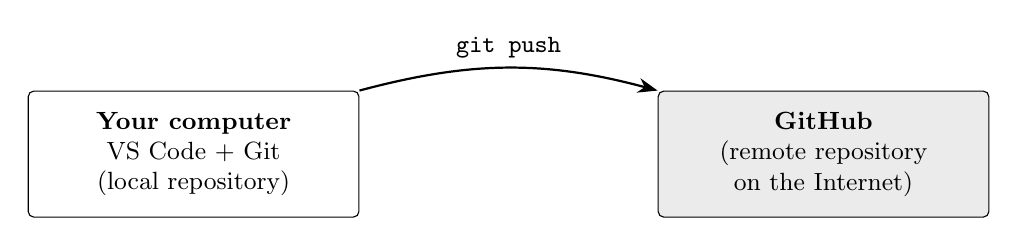
\begin{tikzpicture}
\node[box,minimum width=4.2cm,minimum height=1.6cm] (pc) at (0,0) {\textbf{Your computer}\\VS Code + Git\\(local repository)};
\node[box,minimum width=4.2cm,minimum height=1.6cm,fill=black!8] (gh) at (8,0) {\textbf{GitHub}\\(remote repository\\on the Internet)};
\draw[arr] (pc.north east) to[bend left=15] node[above,font=\small]{\code{git push}} (gh.north west);
\end{tikzpicture}
\figcap{Figure 1: Git works on your computer; GitHub stores a copy online}
\end{center}

\textbf{Key terms:}
\begin{itemize}
\item \textbf{Repository (repo):} A project folder whose history is tracked by Git.
\item \textbf{Commit:} A saved snapshot of your files, with a message describing the change.
\item \textbf{Branch:} A line of development. Our main branch is called \code{main}.
\item \textbf{Remote:} A copy of the repository stored on another computer, such as GitHub.
\end{itemize}

%=========================================================
\section{Installing VS Code (Windows)}
%=========================================================

\begin{enumerate}
\item Open a web browser and go to \code{https://code.visualstudio.com}.
\item Click \menu{Download for Windows}. The installer file (e.g., \code{VSCodeUserSetup-x64-\ldots.exe}) is downloaded.
\item Double-click the downloaded file to start the installer.
\item \textbf{License Agreement:} Select \menu{I accept the agreement} and click \menu{Next}.
\item \textbf{Select Destination Location:} Keep the default folder and click \menu{Next}.
\item \textbf{Select Start Menu Folder:} Keep the default and click \menu{Next}.
\item \textbf{Select Additional Tasks:} Tick the following options and click \menu{Next}:
  \begin{itemize}
  \item Create a desktop icon.
  \item Add ``Open with Code'' action to Windows Explorer file context menu.
  \item Add ``Open with Code'' action to Windows Explorer directory context menu.
  \item Register Code as an editor for supported file types.
  \item \textbf{Add to PATH} (keep this ticked; it lets you type \code{code} in a terminal).
  \end{itemize}
\item Click \menu{Install} and wait for the installation to finish.
\item Tick \menu{Launch Visual Studio Code} and click \menu{Finish}.
\end{enumerate}

\begin{notebox}
The installer screens may look slightly different in newer versions. If an option is not mentioned above, keep its default value.
\end{notebox}

%=========================================================
\section{Installing Git (Windows)}
%=========================================================

\begin{enumerate}
\item Go to \code{https://git-scm.com} and click \menu{Download for Windows}.
\item Download the \textbf{64-bit Git for Windows Setup} file and double-click it.
\item \textbf{Information (license):} Click \menu{Next}.
\item \textbf{Select Destination Location:} Keep the default and click \menu{Next}.
\item \textbf{Select Components:} Keep the defaults and click \menu{Next}.
\item \textbf{Choosing the default editor used by Git:} Select \menu{Use Visual Studio Code as Git's default editor} and click \menu{Next}.
\item \textbf{Adjusting the name of the initial branch in new repositories:} Select \menu{Override the default branch name for new repositories} and make sure the name is \code{main}. Click \menu{Next}.
\item \textbf{Adjusting your PATH environment:} Keep \menu{Git from the command line and also from 3rd-party software} (recommended) and click \menu{Next}.
\item For all the remaining screens, keep the default options and click \menu{Next}.
\item Click \menu{Install}, then \menu{Finish}.
\end{enumerate}

\begin{notebox}[Why set the branch name to main?]
We push our work using \code{git push origin main}. If Git names the first branch \code{master} instead, this command fails. Setting the default branch to \code{main} during installation avoids this problem. (If you missed this step, see Section~\ref{sec:errors}.)
\end{notebox}

\subsection{Verify the Installation}

Close and reopen VS Code (so that it picks up the new PATH), open the terminal (\menu{Terminal} $\rightarrow$ \menu{New Terminal}), and type:

\begin{cmd}
git --version
\end{cmd}
\begin{outbox}
git version 2.xx.x.windows.1
\end{outbox}

Any version number means Git is installed correctly. (The exact number depends on the version you downloaded.)

%=========================================================
\section{A Tour of the VS Code Window}
%=========================================================

\begin{center}
\begin{tikzpicture}
\node[anchor=south west,inner sep=0] (img) at (0,0) {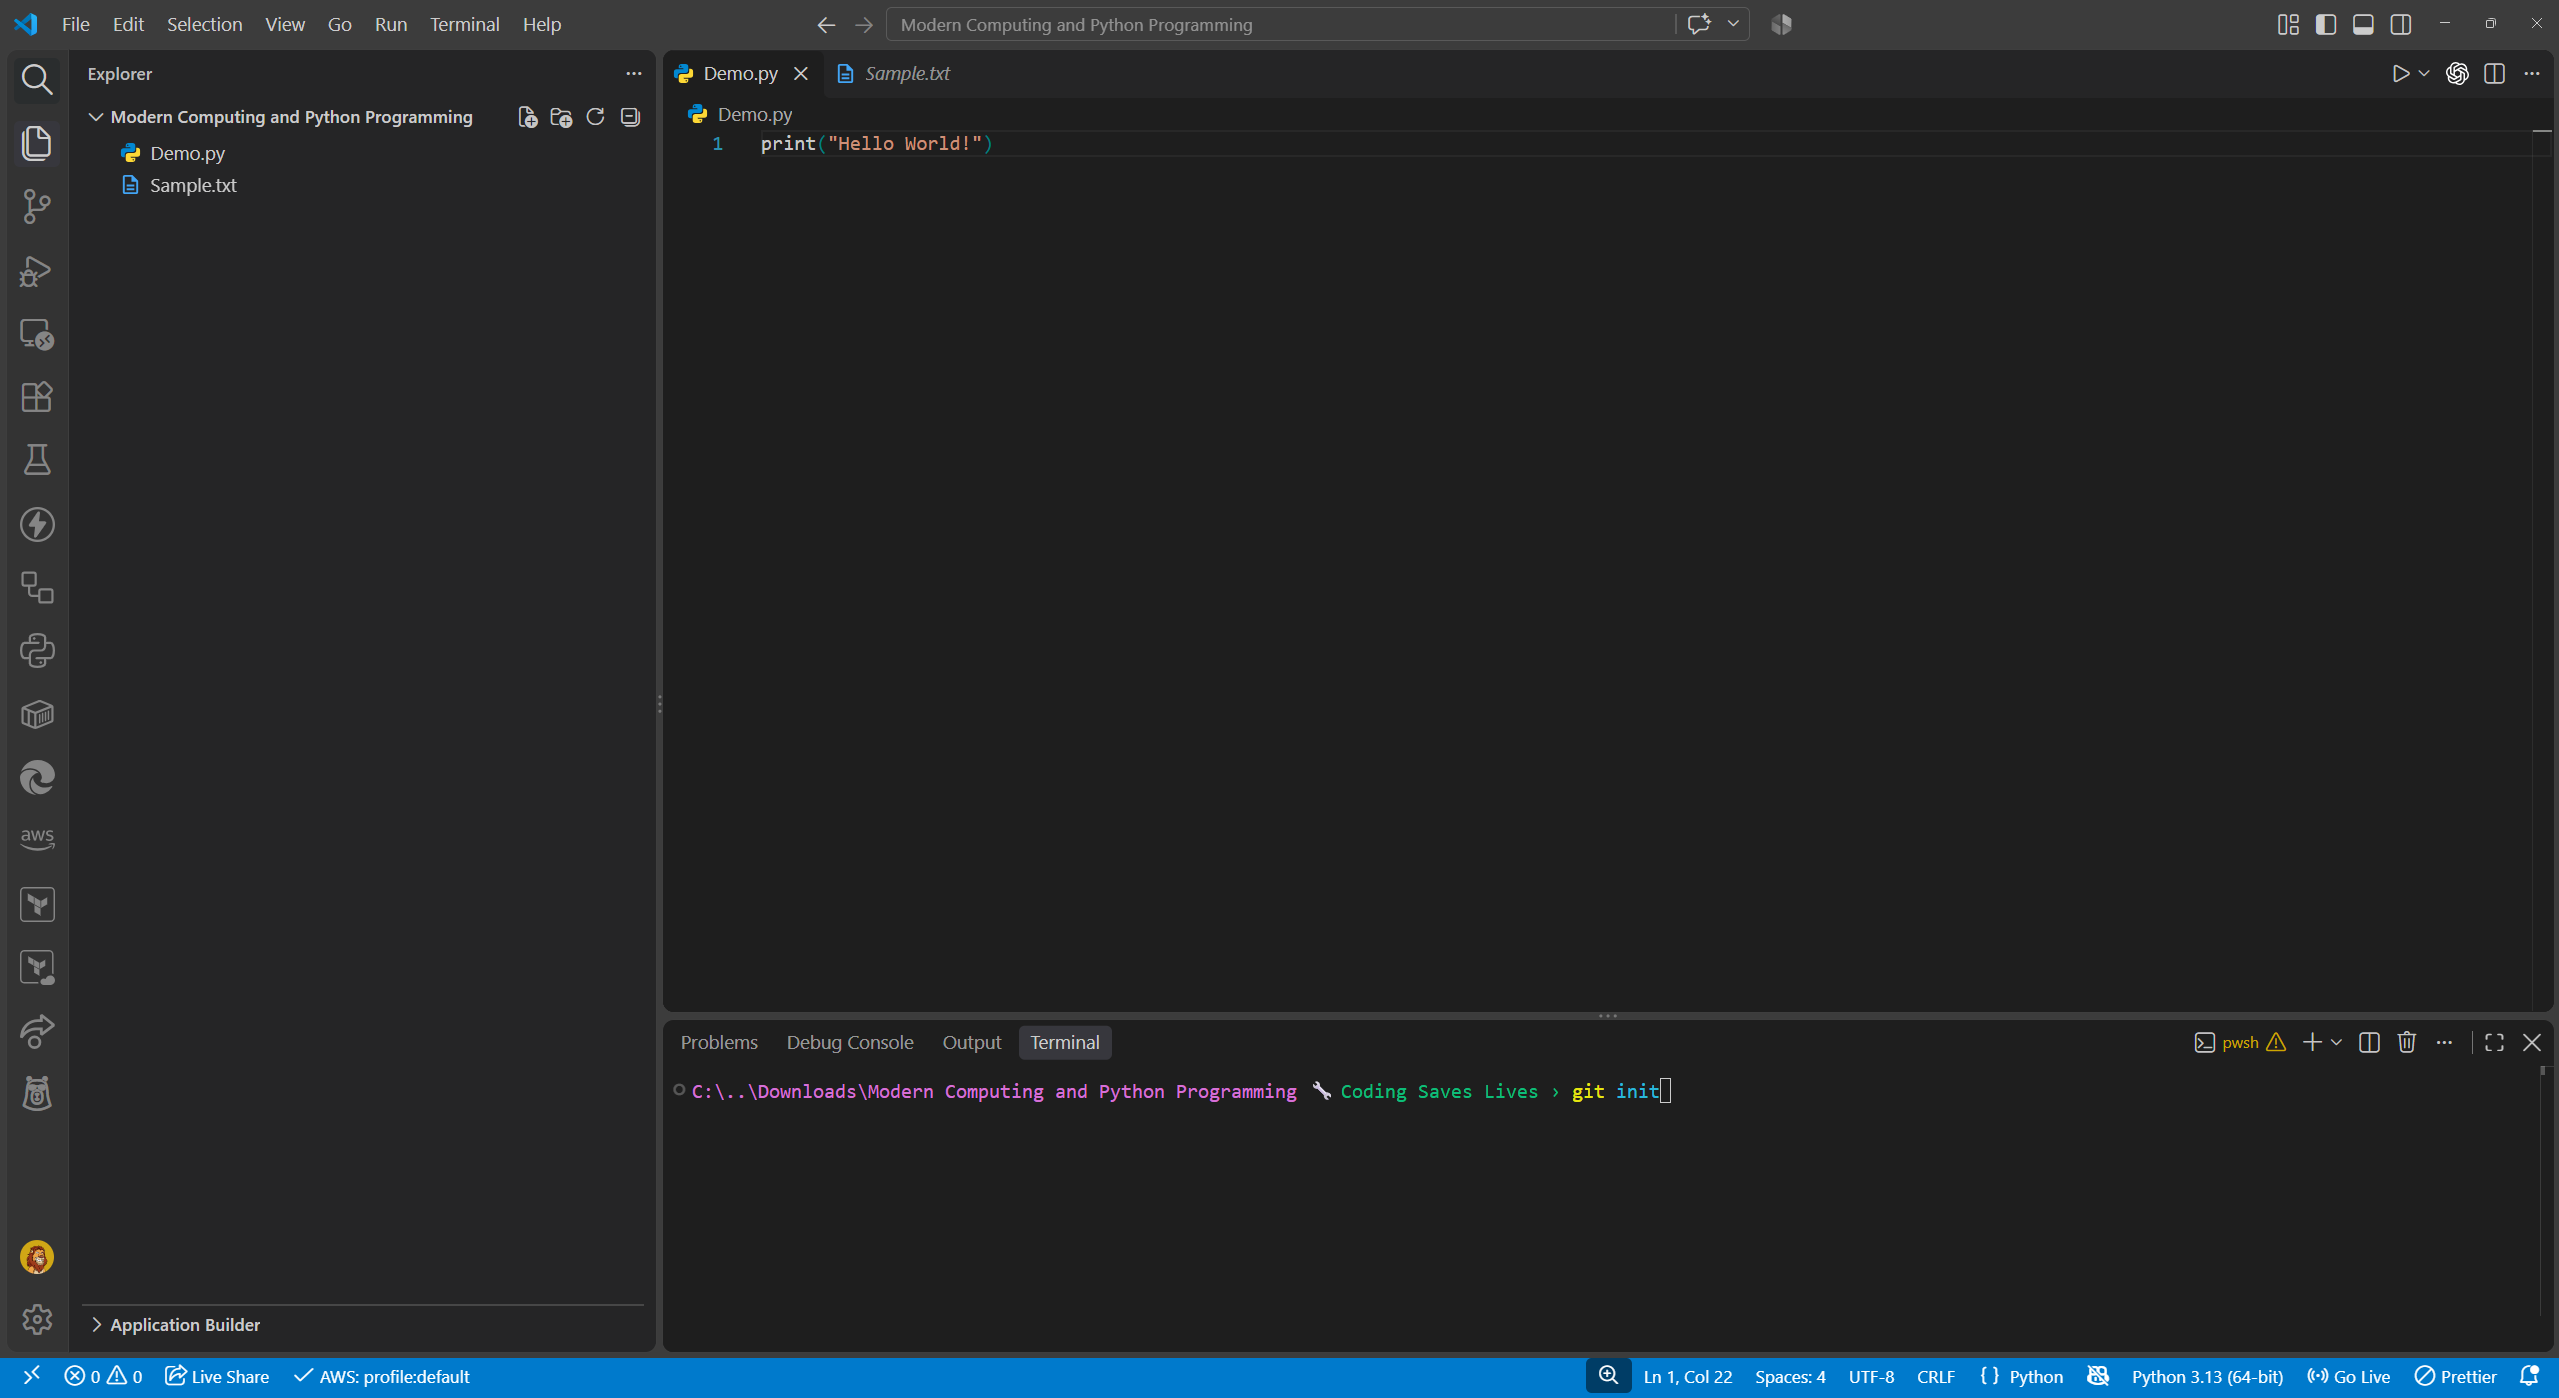
\includegraphics[width=0.85\linewidth]{images/vscode_window.png}};
\begin{scope}[x={(img.south east)},y={(img.north west)}]
\draw[red,line width=1.1pt,rounded corners=1pt] (0.0203,0.9971) rectangle (0.2235,0.9671);
\draw[red,line width=1.1pt,rounded corners=1pt] (0.0008,0.9628) rectangle (0.0274,0.0329);
\draw[red,line width=1.1pt,rounded corners=1pt] (0.0289,0.9628) rectangle (0.2564,0.0329);
\draw[red,line width=1.1pt,rounded corners=1pt] (0.2587,0.9628) rectangle (0.9984,0.2775);
\draw[red,line width=1.1pt,rounded corners=1pt] (0.2587,0.2718) rectangle (0.9984,0.0315);
\draw[red,line width=1.1pt,rounded corners=1pt] (0.0008,0.0286) rectangle (0.9992,0.0007);
\node[callout] at (0.2501,0.9821) {1};
\node[callout] at (0.0141,0.1631) {2};
\node[callout] at (0.1426,0.4850) {3};
\node[callout] at (0.6252,0.5994) {4};
\node[callout] at (0.6252,0.1130) {5};
\node[callout] at (0.4377,0.0143) {6};
\draw[red,thick,-{Stealth[length=1.6mm]}] (-0.0120,0.9428) -- (0.0055,0.9428);
\node[anchor=east,font=\scriptsize\bfseries,inner sep=1pt] at (-0.0120,0.9428) {Search};
\draw[red,thick,-{Stealth[length=1.6mm]}] (-0.0120,0.8984) -- (0.0055,0.8984);
\node[anchor=east,font=\scriptsize\bfseries,inner sep=1pt] at (-0.0120,0.8984) {Explorer};
\draw[red,thick,-{Stealth[length=1.6mm]}] (-0.0120,0.8534) -- (0.0055,0.8534);
\node[anchor=east,font=\scriptsize\bfseries,inner sep=1pt] at (-0.0120,0.8534) {Source Control};
\draw[red,thick,-{Stealth[length=1.6mm]}] (-0.0120,0.8069) -- (0.0055,0.8069);
\node[anchor=east,font=\scriptsize\bfseries,inner sep=1pt] at (-0.0120,0.8069) {Run and Debug};
\draw[red,thick,-{Stealth[length=1.6mm]}] (-0.0120,0.7160) -- (0.0055,0.7160);
\node[anchor=east,font=\scriptsize\bfseries,inner sep=1pt] at (-0.0120,0.7160) {Extensions};
\draw[red,thick,-{Stealth[length=1.6mm]}] (-0.0120,0.1001) -- (0.0055,0.1001);
\node[anchor=east,font=\scriptsize\bfseries,inner sep=1pt] at (-0.0120,0.1001) {Accounts};
\draw[red,thick,-{Stealth[length=1.6mm]}] (-0.0120,0.0558) -- (0.0055,0.0558);
\node[anchor=east,font=\scriptsize\bfseries,inner sep=1pt] at (-0.0120,0.0558) {Manage};
\end{scope}
\end{tikzpicture}
\figcap{Figure 2: Main parts of the VS Code window --- \textcircled{\scriptsize 1} Menu bar, \textcircled{\scriptsize 2} Activity bar, \textcircled{\scriptsize 3} Side bar (Explorer), \textcircled{\scriptsize 4} Editor, \textcircled{\scriptsize 5} Panel with the integrated terminal, \textcircled{\scriptsize 6} Status bar}
\end{center}

\begin{enumerate}
\item \textbf{Menu bar:} The row of menus at the top: \menu{File}, \menu{Edit}, \menu{Selection}, \menu{View}, \menu{Go}, \menu{Run}, \menu{Terminal}, \menu{Help}. For example, \menu{File} $\rightarrow$ \menu{Open Folder} opens a project folder, and \menu{Terminal} $\rightarrow$ \menu{New Terminal} opens the terminal.
\item \textbf{Activity bar:} The narrow vertical bar of icons on the far left. Clicking an icon changes what the side bar shows. (Extra icons appear when you install extensions, e.g., Testing, Python, or AWS in Figure 2, and the order of icons can differ from computer to computer.)
  \begin{itemize}
  \item \textbf{Explorer} (\code{Ctrl+Shift+E}): shows the files and folders of the opened project.
  \item \textbf{Search} (\code{Ctrl+Shift+F}): searches for text across all files.
  \item \textbf{Source Control} (\code{Ctrl+Shift+G}): the Git panel; shows \textbf{Changes} and \textbf{Staged Changes} and lets you commit.
  \item \textbf{Run and Debug} (\code{Ctrl+Shift+D}): runs and debugs programs.
  \item \textbf{Extensions} (\code{Ctrl+Shift+X}): installs add-ons such as the \textbf{Python} extension.
  \item \textbf{Accounts} and \textbf{Manage} (bottom): sign in (e.g., to GitHub) and open settings.
  \end{itemize}
\item \textbf{Side bar:} The panel next to the activity bar. Its content depends on the activity bar icon selected (Explorer, Source Control, etc.).
\item \textbf{Editor:} The large central area where you open and edit files. Each open file appears as a tab (e.g., \code{Demo.py} and \code{Sample.txt} in Figure 2).
\item \textbf{Panel with the integrated terminal:} The area at the bottom, with the tabs \textbf{Problems}, \textbf{Debug Console}, \textbf{Output}, and \textbf{Terminal}. The \textbf{Terminal} tab runs \textbf{PowerShell} (shown as \code{pwsh} or \code{powershell}; the default terminal on Windows) inside VS Code, so you can type Git commands without leaving the editor. Open it with \menu{Terminal} $\rightarrow$ \menu{New Terminal} or \code{Ctrl+`} (backtick).
\item \textbf{Status bar:} The thin bar at the very bottom. It shows errors and warnings, the cursor position (e.g., \code{Ln 1, Col 22}), the file's language (\code{Python}), and the Python version. Once the folder is a Git repository, it also shows the current branch (e.g., \code{main}).
\end{enumerate}

\subsection{Open a Project Folder}

Git works on a \textbf{folder}. Before using Git, open your project folder in VS Code:
\begin{enumerate}
\item Create a folder, for example \code{C:\textbackslash Users\textbackslash Student\textbackslash MCPP}.
\item In VS Code, select \menu{File} $\rightarrow$ \menu{Open Folder\ldots}, choose the folder, and click \menu{Select Folder}. If asked, click \menu{Yes, I trust the authors}.
\item Create a file, e.g., \code{hello.py}, using the \menu{New File} icon in the Explorer, and save it (\code{Ctrl+S}).
\item Open the terminal (\code{Ctrl+`}). The prompt shows that you are inside your folder:
\end{enumerate}
\begin{outbox}
PS C:\Users\Student\MCPP>
\end{outbox}

%=========================================================
\section{Creating a GitHub Account and Signing In}
\label{sec:account}
%=========================================================

\subsection{Sign Up (Create an Account)}

\begin{enumerate}
\item Open \code{https://github.com} and click \menu{Sign up} (top-right).
\item Enter your \textbf{email address}. Use an email you can open now, because GitHub sends a verification code to it.
\item Create a \textbf{password}. Use a strong password and do not share it.
\item Choose a \textbf{username}. It becomes part of every repository address, e.g., \code{github.com/\allowbreak<username>/\allowbreak<repository>}, so choose a simple, professional name (e.g., your first and last name).
\item Select your \textbf{country/region} and email preferences, then click \menu{Create account} (or \menu{Continue}).
\item Complete the \textbf{verification puzzle} that checks that you are a human.
\item Open your email inbox, copy the \textbf{launch code} sent by GitHub, and enter it on the GitHub page.
\item Your account is now created. If GitHub asks optional questions about how you will use it, you may answer them or skip them. Choose the \textbf{Free} plan if a plan is offered.
\end{enumerate}

\subsection{Sign In (Log In)}

\begin{enumerate}
\item Open \code{https://github.com} and click \menu{Sign in}.
\item Enter your \textbf{username or email address} and your \textbf{password}, and click \menu{Sign in}.
\item If GitHub asks for \textbf{device verification}, enter the code sent to your email.
\item If GitHub asks you to set up \textbf{two-factor authentication (2FA)}, follow the on-screen steps using an authenticator app on your phone, and \textbf{save the recovery codes} in a safe place.
\item When you are signed in, your profile picture (avatar) appears at the top-right of every GitHub page.
\end{enumerate}

\begin{notebox}
GitHub changes its sign-up screens from time to time, so the exact wording may differ slightly. The information asked for (email, password, username, verification) remains the same.
\end{notebox}

%=========================================================
\section{How Git Tracks Your Work}
%=========================================================

Git moves your changes through \textbf{three local areas} and then to the \textbf{remote} repository on GitHub.

\begin{center}
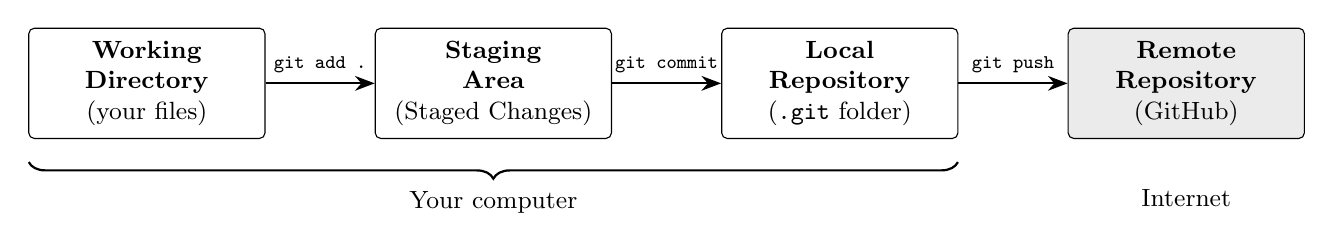
\begin{tikzpicture}
\node[box,minimum width=3cm,minimum height=1.4cm] (wd) at (0,0) {\textbf{Working}\\\textbf{Directory}\\(your files)};
\node[box,minimum width=3cm,minimum height=1.4cm] (st) at (4.4,0) {\textbf{Staging}\\\textbf{Area}\\(Staged Changes)};
\node[box,minimum width=3cm,minimum height=1.4cm] (lr) at (8.8,0) {\textbf{Local}\\\textbf{Repository}\\(\code{.git} folder)};
\node[box,minimum width=3cm,minimum height=1.4cm,fill=black!8] (rr) at (13.2,0) {\textbf{Remote}\\\textbf{Repository}\\(GitHub)};
\draw[arr] (wd)--node[above,font=\scriptsize]{\code{git add .}} (st);
\draw[arr] (st)--node[above,font=\scriptsize]{\code{git commit}} (lr);
\draw[arr] (lr)--node[above,font=\scriptsize]{\code{git push}} (rr);
\draw[decorate,decoration={brace,amplitude=6pt,mirror},thick] (-1.5,-1.0)--(10.3,-1.0) node[midway,below=7pt,font=\small]{Your computer};
\node[font=\small] at (13.2,-1.45) {Internet};
\end{tikzpicture}
\figcap{Figure 3: The path of a change --- working directory $\rightarrow$ staging area $\rightarrow$ local repository $\rightarrow$ GitHub}
\end{center}

\begin{enumerate}
\item \textbf{Working directory:} The files you see and edit in the Explorer. Edited files appear under \textbf{Changes} in the Source Control panel.
\item \textbf{Staging area:} A waiting area for the changes you want to include in the next commit. Staged files appear under \textbf{Staged Changes}.
\item \textbf{Local repository:} The hidden \code{.git} folder in your project, where Git stores every commit.
\item \textbf{Remote repository:} The copy of your repository on GitHub.
\end{enumerate}

%=========================================================
\section{Git Commands, Step by Step}
%=========================================================

Type each command in the VS Code terminal \textbf{inside your project folder} and press \code{Enter}.

%---------------------------------------------------------
\subsection{Step 1: \code{git init} --- Create a Repository}

\textbf{Purpose:} Turns the current folder into a Git repository. Git creates a hidden \code{.git} folder in which it will store the history of the project. Run it \textbf{once per project}.

\begin{cmd}
git init
\end{cmd}
\begin{outbox}
Initialized empty Git repository in C:/Users/Student/MCPP/.git/
\end{outbox}

After this, the Source Control icon in the activity bar shows a number: the count of files that Git has noticed.

%---------------------------------------------------------
\subsection{Step 2: \code{git config} --- Tell Git Who You Are}

\textbf{Purpose:} Every commit records the \textbf{name} and \textbf{email} of its author. Set them \textbf{once per computer}; the \code{--global} option applies them to all repositories on that computer.

\begin{cmd}
git config --global user.name "Your Name"
git config --global user.email "your.email@example.com"
\end{cmd}

These commands print nothing when they succeed. To check the values you have set:

\begin{cmd}
git config --global --list
\end{cmd}
\begin{outbox}
user.name=Your Name
user.email=your.email@example.com
\end{outbox}

\begin{notebox}
Use the \textbf{same email address} as your GitHub account, so that GitHub links the commits to your profile. Put the name in double quotes because it contains a space.
\end{notebox}

%---------------------------------------------------------
\subsection{Step 3: \code{git add .} --- Stage the Changes}

\textbf{Purpose:} Moves all new and modified files from \textbf{Changes} to \textbf{Staged Changes}, i.e., prepares them for the next commit. The dot (\code{.}) means ``everything in the current folder''.

\begin{cmd}
git add .
\end{cmd}

This command normally prints nothing. On Windows you may see a harmless warning such as \code{LF will be replaced by CRLF}; it can be ignored.

In the Source Control panel, the files now move from \textbf{Changes} to \textbf{Staged Changes}.

%---------------------------------------------------------
\subsection{Step 4: \code{git commit -m "message"} --- Save a Snapshot}

\textbf{Purpose:} Permanently records the staged changes in the local repository as a \textbf{commit}. The \code{-m} option supplies a short message describing what you changed.

\begin{cmd}
git commit -m "Add hello.py program"
\end{cmd}
\begin{outbox}
[main (root-commit) 3f2a9c1] Add hello.py program
 1 file changed, 1 insertion(+)
 create mode 100644 hello.py
\end{outbox}

\begin{itemize}
\item \code{main} is the branch name; \code{root-commit} means this is the first commit.
\item \code{3f2a9c1} is the short commit ID (yours will be different).
\item After committing, the \textbf{Staged Changes} list in the Source Control panel becomes empty.
\end{itemize}

\begin{notebox}[Writing good commit messages]
Write a short message that says \textbf{what} changed, e.g., \code{"Add factorial program"} or \code{"Fix input bug in marks.py"}. Avoid messages such as \code{"update"} or \code{"done"}.
\end{notebox}

%---------------------------------------------------------
\subsection{Step 5: Create an Empty Repository on GitHub}

Before connecting your project to GitHub, a repository must exist there:
\begin{enumerate}
\item Sign in at \code{https://github.com} (Section~\ref{sec:account}).
\item Click \menu{+} (top-right) $\rightarrow$ \menu{New repository}.
\item Enter a \textbf{Repository name} (e.g., \code{Modern-Computing-and-Python-Programming}). Use hyphens instead of spaces.
\item Optionally, type a short \textbf{Description} of the project.
\item Choose \menu{Public} (anyone can see it) or \menu{Private} (only you and the people you invite can see it).
\item \textbf{Do not} add a README file, a \code{.gitignore}, or a license --- the repository must be \textbf{empty}, because your files will come from your computer.
\item Click \menu{Create repository}.
\item GitHub opens a \textbf{Quick setup} page. Make sure \menu{HTTPS} is selected and copy the URL shown, which ends in \code{.git}. You will use it in Step 6.
\end{enumerate}

%---------------------------------------------------------
\subsection{Step 6: \code{git remote} --- Connect to GitHub}

\textbf{Purpose:} \code{git remote add} gives a short name to the GitHub repository's URL. By convention the name is \code{origin}.

\begin{cmd}
git remote add origin https://github.com/ManjunathPrasad/Modern-Computing-and-Python-Programming.git
\end{cmd}

\textbf{Replace the URL with the URL of your own repository.} This command prints nothing when it succeeds.

To list the remotes that are connected:

\begin{cmd}
git remote
\end{cmd}
\begin{outbox}
origin
\end{outbox}

To see the remote names together with their URLs, add \code{-v} (verbose):

\begin{cmd}
git remote -v
\end{cmd}
\begin{outbox}
origin  https://github.com/ManjunathPrasad/Modern-Computing-and-Python-Programming.git (fetch)
origin  https://github.com/ManjunathPrasad/Modern-Computing-and-Python-Programming.git (push)
\end{outbox}

%---------------------------------------------------------
\subsection{Step 7: \code{git push origin main} --- Upload to GitHub}

\textbf{Purpose:} Sends the commits of the local \code{main} branch to the remote named \code{origin} (GitHub).

\begin{cmd}
git push origin main
\end{cmd}

\textbf{First push only:} A window titled \textbf{Connect to GitHub} appears. Click \menu{Sign in with your browser}, log in to GitHub, and click \menu{Authorize}. Git remembers this login, so you will not be asked again on the same computer.

\begin{outbox}
Enumerating objects: 3, done.
Counting objects: 100% (3/3), done.
Writing objects: 100% (3/3), 245 bytes | 245.00 KiB/s, done.
Total 3 (delta 0), reused 0 (delta 0), pack-reused 0
To https://github.com/ManjunathPrasad/Modern-Computing-and-Python-Programming.git
 * [new branch]      main -> main
\end{outbox}

Refresh the repository page on GitHub: your files and your commit message now appear there. Section~\ref{sec:explore} explains what you see on that page.

%=========================================================
\section{The Complete Workflow}
%=========================================================

\subsection{First Time (New Project)}

\begin{cmd}
git init
git config --global user.name "Your Name"
git config --global user.email "your.email@example.com"
git add .
git commit -m "First commit"
git remote add origin https://github.com/<username>/<repository>.git
git push origin main
\end{cmd}

\subsection{Every Time After That}

Once the project is set up, the daily cycle has only three commands:

\begin{center}
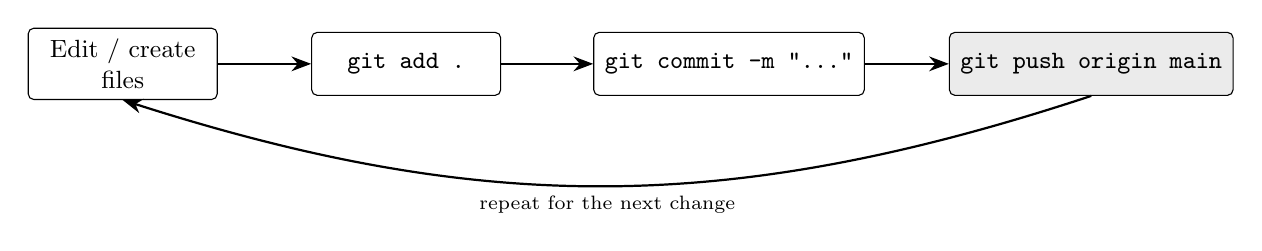
\begin{tikzpicture}
\node[box,minimum width=2.4cm] (e) at (0,0) {Edit / create\\files};
\node[box,minimum width=2.4cm] (a) at (3.6,0) {\code{git add .}};
\node[box] (c) at (7.7,0) {\code{git commit -m "..."}};
\node[box,fill=black!8] (p) at (12.3,0) {\code{git push origin main}};
\draw[arr] (e)--(a); \draw[arr] (a)--(c); \draw[arr] (c)--(p);
\draw[arr] (p.south) to[bend left=18] node[below,font=\scriptsize]{repeat for the next change} (e.south);
\end{tikzpicture}
\figcap{Figure 4: The everyday Git cycle}
\end{center}

\begin{cmd}
git add .
git commit -m "Describe your change"
git push origin main
\end{cmd}

\subsection{The Same Steps Using VS Code Buttons}

The Source Control panel (\code{Ctrl+Shift+G}) can do the same work without typing commands:

\begin{center}
\renewcommand{\arraystretch}{1.3}
\small
\begin{tabularx}{\linewidth}{|l|X|}
\hline
\textbf{Command} & \textbf{Equivalent action in the Source Control panel} \\ \hline
\code{git init} & Click \menu{Initialize Repository} (shown when the folder is not yet a repository). \\ \hline
\code{git add .} & Click the \menu{+} (Stage All Changes) icon next to the \textbf{Changes} heading. \\ \hline
\code{git commit -m "..."} & Type the message in the box at the top and click \menu{Commit}. \\ \hline
\code{git push origin main} & Click \menu{Sync Changes} / \menu{Publish Branch}, or \menu{\ldots} $\rightarrow$ \menu{Push}. \\ \hline
\end{tabularx}
\end{center}

%=========================================================
\section{Exploring Your Repository on GitHub}
\label{sec:explore}
%=========================================================

After a few pushes, open your repository on \code{github.com}. The screenshots below are of the course repository after \textbf{four commits} were pushed.

%---------------------------------------------------------
\subsection{The Repository Home Page}

Address: \code{https://github.com/<username>/<repository>}

\begin{center}
\begin{tikzpicture}
\node[anchor=south west,inner sep=0] (img) at (0,0) {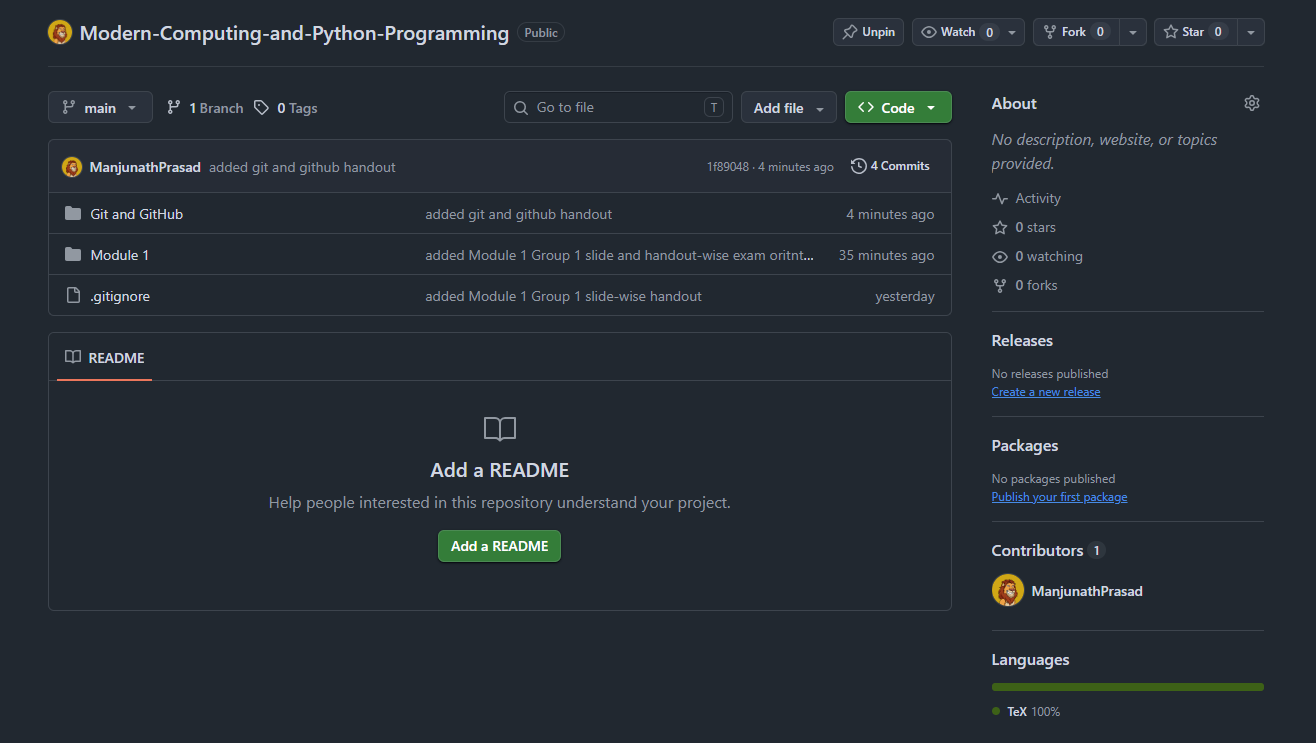
\includegraphics[width=\linewidth]{images/github_repo_home.png}};
\begin{scope}[x={(img.south east)},y={(img.north west)}]
\draw[red,line width=1.1pt,rounded corners=1pt] (0.0320,0.9828) rectangle (0.4320,0.9313);
\draw[red,line width=1.1pt,rounded corners=1pt] (0.0350,0.8797) rectangle (0.1155,0.8333);
\draw[red,line width=1.1pt,rounded corners=1pt] (0.1204,0.8797) rectangle (0.2476,0.8333);
\draw[red,line width=1.1pt,rounded corners=1pt] (0.6388,0.8814) rectangle (0.7243,0.8316);
\draw[red,line width=1.1pt,rounded corners=1pt] (0.0369,0.7973) rectangle (0.6369,0.7543);
\draw[red,line width=1.1pt,rounded corners=1pt] (0.6408,0.7955) rectangle (0.7146,0.7577);
\draw[red,line width=1.1pt,rounded corners=1pt] (0.0369,0.7371) rectangle (0.7214,0.5790);
\draw[red,line width=1.1pt,rounded corners=1pt] (0.0369,0.5533) rectangle (0.7214,0.1804);
\draw[red,line width=1.1pt,rounded corners=1pt] (0.7476,0.8849) rectangle (0.9631,0.0258);
\node[callout] at (0.4466,0.9570) {1};
\node[callout] at (0.0748,0.8076) {2};
\node[callout] at (0.1845,0.8076) {3};
\node[callout] at (0.7379,0.9021) {4};
\node[callout] at (0.3689,0.8144) {5};
\node[callout] at (0.6796,0.8144) {6};
\node[callout] at (0.0223,0.6581) {7};
\node[callout] at (0.0223,0.3694) {8};
\node[callout] at (0.9806,0.8591) {9};
\end{scope}
\end{tikzpicture}
\figcap{Figure 5: Repository home page after four pushes}
\end{center}

\begin{enumerate}
\item \textbf{Repository name and visibility:} The name of the repository and a \textbf{Public} (or \textbf{Private}) label. In the page header, the owner's username (\code{ManjunathPrasad}) appears before the repository name.
\item \textbf{Branch selector:} Shows the branch being viewed (\code{main}). Click it to switch to another branch.
\item \textbf{Branches and tags:} \textbf{1 Branch} shows how many branches the repository has; click it to open the branches page (Figure~6). \textbf{0 Tags} shows that no version has been tagged yet.
\item \textbf{Code button:} Gives the repository URL and a ZIP download (Figure~8).
\item \textbf{Latest commit:} The author (\code{ManjunathPrasad}), the commit message (\code{added git and github handout}), the short commit ID (\code{1f89048}), and how long ago it was pushed.
\item \textbf{Commit count:} \textbf{4 Commits} is the total number of commits on this branch. Click it to open the commit history (Figure~7).
\item \textbf{Files and folders:} The contents of the repository. Each row shows the name, the message of the \textbf{last commit that changed it}, and when. Note that build files such as \code{.aux} and \code{.log} do not appear, because \code{.gitignore} told Git to ignore them.
\item \textbf{README area:} GitHub displays the \code{README.md} file here. This repository has none yet, so GitHub offers an \menu{Add a README} button.
\item \textbf{About sidebar:} The description, stars, watchers, forks, releases, packages, \textbf{contributors} (people who have committed), and \textbf{languages} (detected from the file types; here TeX 100\%).
\end{enumerate}

%---------------------------------------------------------
\subsection{Branches}

Address: \code{https://github.com/<username>/<repository>/branches} (or click \textbf{1 Branch} in Figure~5)

\begin{center}
\begin{tikzpicture}
\node[anchor=south west,inner sep=0] (img) at (0,0) {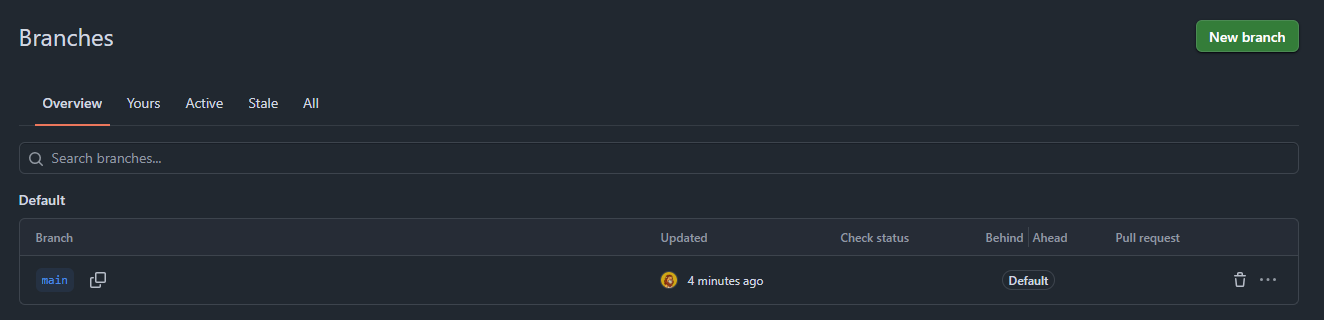
\includegraphics[width=\linewidth]{images/github_branches.png}};
\begin{scope}[x={(img.south east)},y={(img.north west)}]
\draw[red,line width=1.1pt,rounded corners=1pt] (0.0222,0.7360) rectangle (0.2493,0.6040);
\draw[red,line width=1.1pt,rounded corners=1pt] (0.9005,0.9440) rectangle (0.9826,0.8320);
\draw[red,line width=1.1pt,rounded corners=1pt] (0.0242,0.1680) rectangle (0.0580,0.0800);
\draw[red,line width=1.1pt,rounded corners=1pt] (0.4947,0.1680) rectangle (0.5816,0.0800);
\draw[red,line width=1.1pt,rounded corners=1pt] (0.7517,0.1680) rectangle (0.8000,0.0800);
\draw[red,line width=1.1pt,rounded corners=1pt] (0.9275,0.1680) rectangle (0.9681,0.0800);
\node[callout] at (0.2657,0.6800) {1};
\node[callout] at (0.8841,0.8880) {2};
\node[callout] at (0.0242,0.0400) {3};
\node[callout] at (0.5382,0.0400) {4};
\node[callout] at (0.7758,0.0400) {5};
\node[callout] at (0.9478,0.0400) {6};
\end{scope}
\end{tikzpicture}
\figcap{Figure 6: The branches page}
\end{center}

\begin{enumerate}
\item \textbf{Tabs:} \textbf{Overview}, \textbf{Yours}, \textbf{Active}, \textbf{Stale}, and \textbf{All} filter the list of branches.
\item \textbf{New branch:} Creates a new branch on GitHub.
\item \textbf{Branch name:} The repository has one branch, \code{main} --- the branch we pushed with \code{git push origin main}.
\item \textbf{Updated:} When the branch last received a commit, and by whom (avatar).
\item \textbf{Default:} \code{main} is the \textbf{default branch}: GitHub shows it on the home page and uses it unless another branch is chosen. The \textbf{Behind/Ahead} columns compare other branches with the default branch.
\item \textbf{Delete and more options:} The bin icon deletes a branch and \menu{\ldots} shows more actions. (The default branch cannot be deleted.)
\end{enumerate}

%---------------------------------------------------------
\subsection{Commits (History)}

Address: \code{https://github.com/<username>/<repository>/commits/main} (or click \textbf{4 Commits} in Figure~5)

\begin{center}
\begin{tikzpicture}
\node[anchor=south west,inner sep=0] (img) at (0,0) {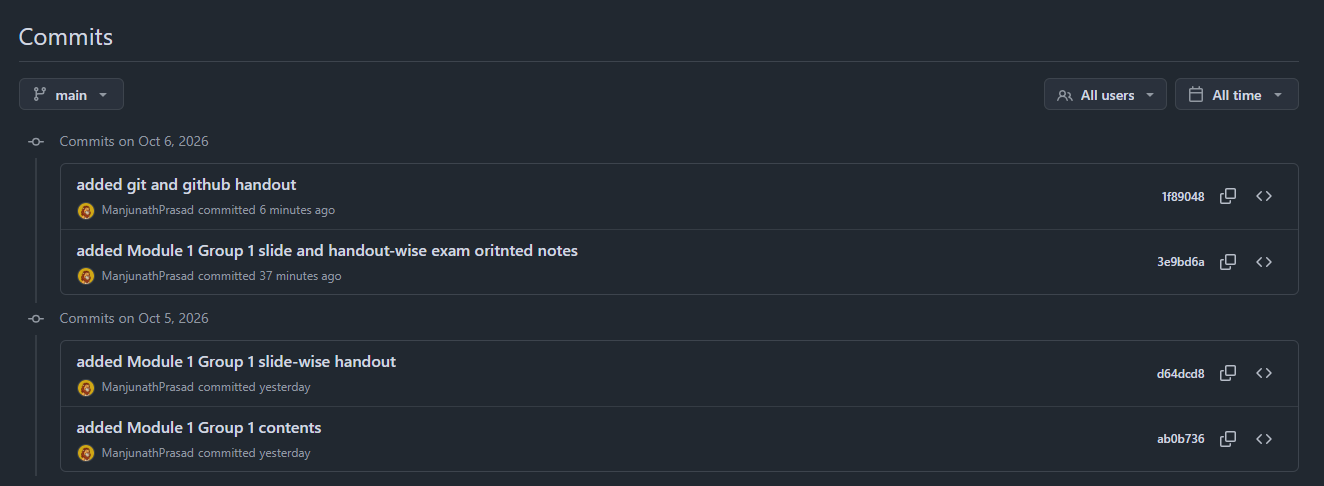
\includegraphics[width=\linewidth]{images/github_commits.png}};
\begin{scope}[x={(img.south east)},y={(img.north west)}]
\draw[red,line width=1.1pt,rounded corners=1pt] (0.0126,0.8421) rectangle (0.0947,0.7711);
\draw[red,line width=1.1pt,rounded corners=1pt] (0.0184,0.7368) rectangle (0.1614,0.6868);
\draw[red,line width=1.1pt,rounded corners=1pt] (0.0551,0.6474) rectangle (0.2280,0.5947);
\draw[red,line width=1.1pt,rounded corners=1pt] (0.0551,0.5921) rectangle (0.2580,0.5474);
\draw[red,line width=1.1pt,rounded corners=1pt] (0.8705,0.6237) rectangle (0.9401,0.5711);
\draw[red,line width=1.1pt,rounded corners=1pt] (0.9430,0.6289) rectangle (0.9662,0.5684);
\node[callout] at (0.1111,0.8079) {1};
\node[callout] at (0.1787,0.7105) {2};
\node[callout] at (0.2464,0.6211) {3};
\node[callout] at (0.2754,0.5684) {4};
\node[callout] at (0.9063,0.5342) {5};
\node[callout] at (0.9807,0.6000) {6};
\end{scope}
\end{tikzpicture}
\figcap{Figure 7: The commit history of the main branch}
\end{center}

\begin{enumerate}
\item \textbf{Branch selector:} The history shown is for the \code{main} branch.
\item \textbf{Date groups:} Commits are grouped by the day they were made (\textbf{Commits on Oct 6, 2026}). The \textbf{newest commit is at the top}.
\item \textbf{Commit message:} Exactly the text given in \code{git commit -m "\ldots"}. Click it to see the changes in that commit: added lines in \textbf{green} and removed lines in \textbf{red}.
\item \textbf{Author and time:} Who made the commit (from \code{git config user.name}) and when.
\item \textbf{Commit ID:} The short commit ID (\code{1f89048}) --- the same ID that \code{git commit} printed in the terminal. The icon next to it copies the full ID.
\item \textbf{Browse files (\code{<>}):} Shows the whole repository as it was at that commit.
\end{enumerate}

\begin{notebox}[Why good commit messages matter]
The commit history is a diary of the project. Clear messages such as \code{added Module 1 Group 1 slide-wise handout} tell everyone what changed in each step without opening the files.
\end{notebox}

%---------------------------------------------------------
\subsection{The Code Button}

\begin{center}
\begin{tikzpicture}
\node[anchor=south west,inner sep=0] (img) at (0,0) {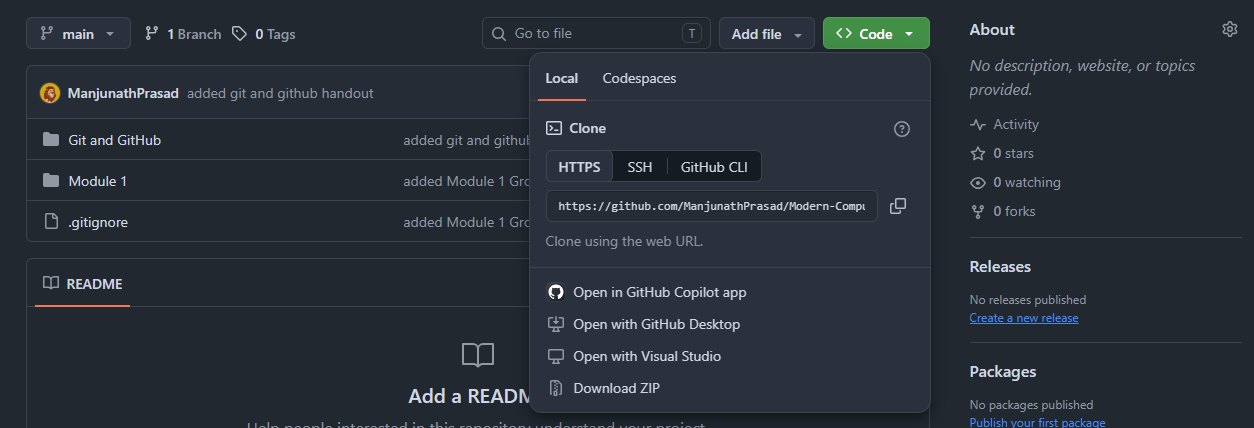
\includegraphics[width=0.85\linewidth]{images/github_code_clone.png}};
\begin{scope}[x={(img.south east)},y={(img.north west)}]
\draw[red,line width=1.1pt,rounded corners=1pt] (0.6541,0.9642) rectangle (0.7429,0.8806);
\draw[red,line width=1.1pt,rounded corners=1pt] (0.4255,0.8537) rectangle (0.4714,0.7701);
\draw[red,line width=1.1pt,rounded corners=1pt] (0.4337,0.6478) rectangle (0.4918,0.5731);
\draw[red,line width=1.1pt,rounded corners=1pt] (0.4337,0.5612) rectangle (0.7286,0.4776);
\draw[red,line width=1.1pt,rounded corners=1pt] (0.4337,0.1254) rectangle (0.5327,0.0657);
\node[callout] at (0.7602,0.9224) {1};
\node[callout] at (0.4133,0.8119) {2};
\node[callout] at (0.4133,0.6119) {3};
\node[callout] at (0.7500,0.5194) {4};
\node[callout] at (0.5510,0.0955) {5};
\end{scope}
\end{tikzpicture}
\figcap{Figure 8: The Code button menu}
\end{center}

\begin{enumerate}
\item \textbf{Code button:} The green button on the repository home page.
\item \textbf{Local tab:} Options for getting the code onto your own computer. (\textbf{Codespaces} opens the code in an online editor instead.)
\item \textbf{HTTPS tab:} Select HTTPS --- the same type of URL used in this handout.
\item \textbf{Repository URL and copy button:} The URL ending in \code{.git}. This is the URL used in \code{git remote add origin <URL>}. Click the copy icon to copy it.
\item \textbf{Download ZIP:} Downloads all the files as a single ZIP file (without the Git history).
\end{enumerate}

%---------------------------------------------------------
\subsection{Demonstration: Watching a Push Appear on GitHub}

\begin{enumerate}
\item Open the repository home page (Figure~5) and note the number of commits (e.g., \textbf{4 Commits}).
\item In VS Code, edit a file or add a new one, and save it.
\item In the terminal, run:
\end{enumerate}
\begin{cmd}
git add .
git commit -m "Add sum.py program"
git push origin main
\end{cmd}
\begin{enumerate}[resume]
\item Refresh the GitHub page. The commit count increases by one (\textbf{5 Commits}), and the latest-commit row shows the new message.
\item Click the commit count. The new commit is at the top of the history (Figure~7), with the same commit ID that the terminal printed.
\item Click the commit message to see exactly which lines were added or changed.
\item Open \textbf{1 Branch} (Figure~6): the \textbf{Updated} time of \code{main} has changed to ``now''.
\end{enumerate}

%=========================================================
\section{Common Errors and How to Fix Them}
\label{sec:errors}
%=========================================================

\begin{center}
\renewcommand{\arraystretch}{1.35}
\small
\begin{tabularx}{\linewidth}{|p{5.3cm}|X|}
\hline
\textbf{Error message} & \textbf{Cause and fix} \\ \hline
\code{git : The term 'git' is not recognized\ldots} & Git is not installed, or VS Code was open during installation. Close and reopen VS Code (or restart the computer) and try again. \\ \hline
\code{fatal: not a git repository} & You are not inside a repository. Check the folder in the prompt, open the correct folder, or run \code{git init}. \\ \hline
\code{Author identity unknown \ldots Please tell me who you are.} & The name and email are not set. Run the two \code{git config --global} commands (Step 2). \\ \hline
\code{nothing to commit, working tree clean} & No changes since the last commit. Edit and \textbf{save} a file first, then run \code{git add .} again. \\ \hline
\code{error: src refspec main does not match any} & Either no commit has been made yet, or your branch is called \code{master}. Make a commit first; if the status bar shows \code{master}, rename the branch with \code{git branch -M main}, then push again. \\ \hline
\code{error: remote origin already exists.} & \code{origin} was added earlier. To change its URL, run \code{git remote set-url origin <new-URL>}. \\ \hline
\code{! [rejected] main -> main (fetch first)} & The GitHub repository already contains files (e.g., a README created on the website). Create a new \textbf{empty} repository (Step 5) and add that URL instead. \\ \hline
\code{Authentication failed} / \code{Permission denied} & You are signed in to a different GitHub account, or the URL is wrong. Check the URL with \code{git remote -v} and sign in with the account that owns the repository. \\ \hline
\end{tabularx}
\end{center}

%=========================================================
\section{Quick Reference}
%=========================================================

\begin{center}
\renewcommand{\arraystretch}{1.35}
\small
\begin{tabularx}{\linewidth}{|p{6.4cm}|X|c|}
\hline
\textbf{Command} & \textbf{What it does} & \textbf{How often} \\ \hline
\code{git --version} & Shows the installed Git version & Once \\ \hline
\code{git init} & Makes the current folder a Git repository & Once per project \\ \hline
\code{git config --global user.name "Name"} & Sets the author name for commits & Once per computer \\ \hline
\code{git config --global user.email "email"} & Sets the author email for commits & Once per computer \\ \hline
\code{git config --global --list} & Shows the configured settings & When checking \\ \hline
\code{git add .} & Stages all changes (Changes $\rightarrow$ Staged Changes) & Every change \\ \hline
\code{git commit -m "message"} & Saves the staged changes as a commit & Every change \\ \hline
\code{git remote} / \code{git remote -v} & Lists remotes (with URLs when \code{-v} is used) & When checking \\ \hline
\code{git remote add origin <URL>} & Connects the repository to GitHub & Once per project \\ \hline
\code{git push origin main} & Uploads commits to GitHub & Every change \\ \hline
\end{tabularx}
\end{center}

%=========================================================
\section{Practice Exercise}
%=========================================================

\begin{enumerate}
\item Create a folder named \code{MCPP-Lab} and open it in VS Code.
\item Create a file \code{hello.py} containing \code{print("Hello, MITE")} and save it.
\item Run \code{git init} and observe the \code{.git} message.
\item Set your name and email with \code{git config --global} and verify them with \code{git config --global --list}.
\item Run \code{git add .} and observe the file moving to \textbf{Staged Changes} in the Source Control panel.
\item Commit with the message \code{"Add hello program"}.
\item Create an empty repository named \code{MCPP-Lab} on GitHub.
\item Connect it using \code{git remote add origin <your-URL>} and check it with \code{git remote -v}.
\item Push using \code{git push origin main} and confirm that \code{hello.py} appears on GitHub.
\item Add a second file \code{sum.py} that prints the sum of two numbers. Add, commit, and push it, and check that GitHub now shows \textbf{2 Commits}.
\item On GitHub, open \textbf{2 Commits} and identify the commit ID, message, author, and time of each commit. Compare the IDs with the ones printed by \code{git commit} in your terminal.
\item Open the branches page and confirm that \code{main} is the \textbf{Default} branch and shows the latest update time.
\end{enumerate}

\end{document}
